\section{Machine Vision}
\subsection{Emperical tests}
This section contains the results of emperical experiments to determine the accuracy of optical distance measurements.
\subsubsection{Experimental setup}
Our experiment consists of two data sets. The first data set is a 2 minute hand-held video footage pointing at the marker that has been measured beforehand at 7 metres away, while the second is a marker at 3 metres away. To illuminate the marker a single 40w incandescent bulb was used at 1.8 metres away from the subject, which yields approximately 14 lux of illuminance. To put it into perspective, a typical library will have an illumination of 500 lux.
\subsubsection{7 Metres away}
The distance approximations the program made for the duration of the 2 minute footage was collected for further statistical analysis. Below follows the result.
\begin{verbatim}
Mean:	7.083622663633182
Standard Error:	0.0026907757522701913
Median:	7.09145
Mode:	6.91049
Standard Deviation:	0.1438244181066202
Sample Variance:	0.020685463243707895
Kurtosis:	0.41526910901933745
Skewness:	-0.0038121380062097533
Range:	1.1244000000000005
\end{verbatim}
From the above one can see that the approximations are satisfactory. Below follows the distribution of the readings:\par
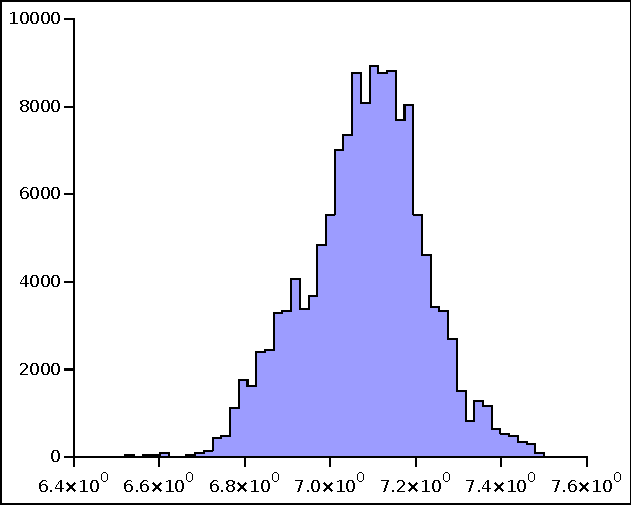
\includegraphics[]{machine_vision/data/7metres.pdf}
\subsubsection{3 Metres away}
In the same vein as the above section we obtained the following statistics for 3 metre approximations.
\begin{verbatim}
Mean:	3.1377264426478018
Standard Error:	0.00032314424822403777
Median:	3.13627
Mode:	3.12397
Standard Deviation:	0.020329857058631336
Sample Variance:	0.0004133030880243824
Kurtosis:	-0.5017583141414064
Skewness:	0.20734696083618784
Range:	0.13027999999999995
\end{verbatim}
\par
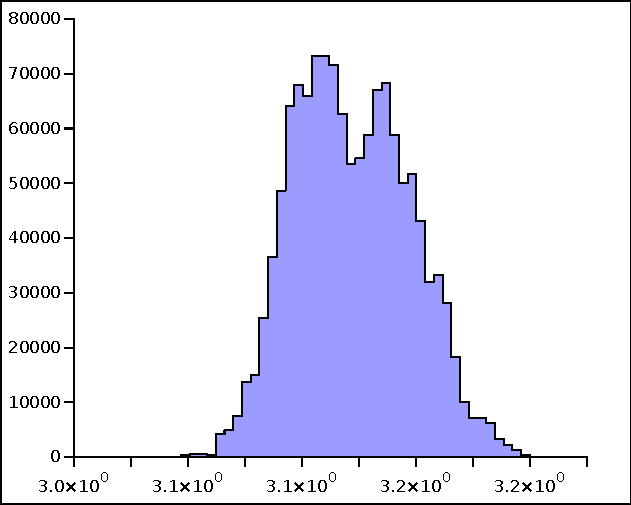
\includegraphics[]{machine_vision/data/3metres.pdf}
\subsection{Automated tests}
All automated tests are implemented under \verb|src/machine_vision/tests|. A single point of entry is provided as a makefile in order to automate the testing of the marker detection algorithm. Testing machine vision has its unique challenges since the test data is visual in nature. Because of this, the tests are constructed around real life video footage, each with distinct challenges to test the system in conditions we expect it to perform poorly. In order to run the battery of tests one must first satisfy the dependencies, that is, the video footage from a google drive. To do this, call \verb|make dependencies|, after which you may call \verb|make tests| to start the battery of tests. During the tests, a window will open showing the video footage as well as an overlay of where the detected tags are and what values they represent. One will also notice some false positives are picked up by the tests. The testing framework will tell you exactly the value of the false positive, in addition the false positive should be visible by inspection during runtime. More on this topic follows below.
\subsection{Remarks on false positives}
On the outdoors test one notices some false positive fiducial marker identification, however it is important to note that it is quite rare. The false positive markers generaly have and id of 17 or 37, which seems to indicate that those particular numbers are encoded in a less robust way. There are a number of remediation strategies that one could employ to reduce the likelihood of false positives or even elimitate them entirely for all intents and purposes. Below follows recommendations for reducing false positive detection.
\subsubsection{Double markers}
Intruducing a second marker allos the system to consider specific pairs of markers as the only valid reading. Any detected marker that is not accompanied by it's partner may be discarded as a false positive. This makes it extremely unlikely for false positives to appear in just the right way so that it is considered a valid reading.
\subsubsection{Emperical elimination of bad tags}
One could peruse campus with a typical camera and record footage in varying environmental conditions and locations. Any markers that are detected are false positives(since the campus is void of any markers at the time of writing this) and are likely less robust as a result. One may construct a list of bad markers and avoid using them altogether.
\subsubsection{Higher bitrate markers}
Aruco, the library we are currently making use of, supports different bitrate markers. The lowest bitrate marker is 4x4 black and white squares, followed by 5x5 and so on and so forth. Increasing the bitrate means that there are far more distinct markers with their own unique embedded hamming codes. This in turn means the that false positive detection rate will drop drastically. However, one trades more robust markers for a shorter detection range.

\section{Backend Unit Test}
For the Backend JUnit and Maven were used

\subsection{Dependencies required}
To set up the tests we had to add dependencies to the pom.xml file. These dependancies made use of JUnit to create and test all unit tests
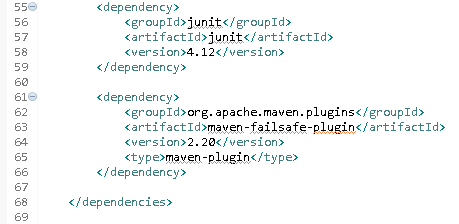
\includegraphics[]{data/backend/Dependencies_needed.png}

\subsection{Setting up Unit Test}
To create the unit test, a standard Java class is created. Inside this class all the 
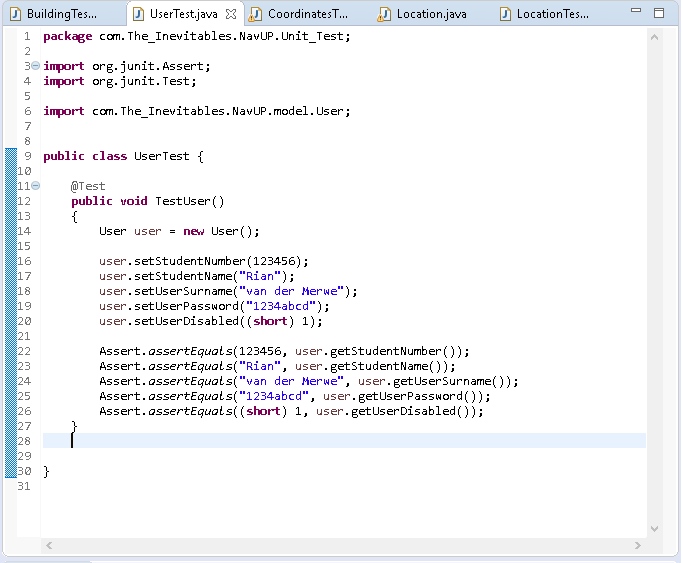
\includegraphics[]{data/backend/User_Unit_Test.png}

\subsection{Running Unit Test}
To execute the unit tests the following command is executed: mvn test. This will compile the project and test all classess annotated as @Test classes

\subsection{Results}
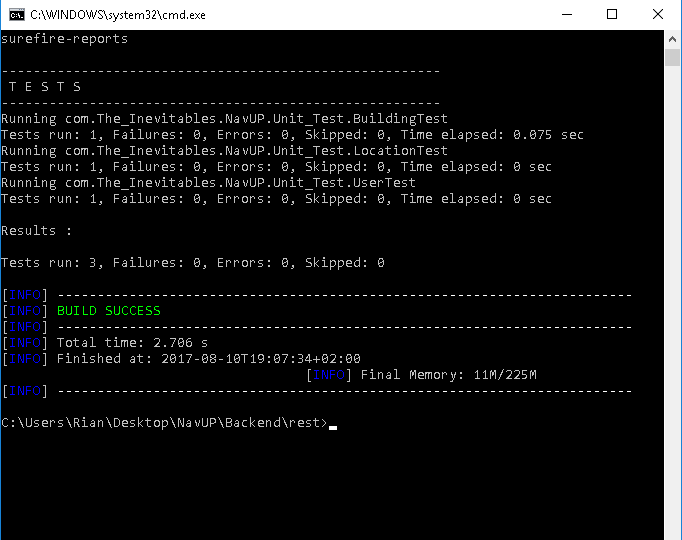
\includegraphics[]{data/backend/Backend_Unit_Tests.png}
